\documentclass[11pt]{article}
\usepackage{upquote}
\usepackage{minted}
\fvset{frame=single}

\usepackage[colorlinks=true]{hyperref}
\usepackage[margin=1in]{geometry}
\usepackage{ifthen}
\usepackage{fancyvrb}

\usepackage{listings}
\usepackage{color}

\definecolor{dkgreen}{rgb}{0,0.6,0}
\definecolor{gray}{rgb}{0.5,0.5,0.5}
\definecolor{mauve}{rgb}{0.58,0,0.82}

\lstset{frame=tb,
  language=Java,
  aboveskip=3mm,
  belowskip=3mm,
  showstringspaces=false,
  columns=flexible,
  basicstyle={\small\ttfamily},
  numbers=none,
  numberstyle=\tiny\color{gray},
  keywordstyle=\color{blue},
  commentstyle=\color{dkgreen},
  stringstyle=\color{mauve},
  breaklines=true,
  breakatwhitespace=true,
  tabsize=3
}

\usepackage{graphicx}
\usepackage{float}

\usepackage{amsmath}
\usepackage{amsfonts}
\usepackage{mathtools}

\usepackage{multirow}
\usepackage{enumitem}

\usepackage{comment}
\usepackage[usenames,dvipsnames,svgnames,table,hyperref]{xcolor}

\newcommand{\vect}[1]{\boldsymbol{#1}}
\newcommand{\matr}[1]{\boldsymbol{#1}}
\DeclareMathOperator*{\argmin}{arg\,min}
\DeclareMathOperator*{\argmax}{arg\,max}
\newcommand{\sol}[1]{{\bf{\color{magenta}{{Solution:}}}}}

\parfillskip=3em plus1fil

\title{CM146, Winter 2023 \\ Problem Set 4: Boosting, Unsupervised learning}
\begin{document}

\author{}
\date{}
\vspace{0in}
\maketitle
\vspace{-0.75in}

\section{AdaBoost}

\subsection{(a)}
\sol x Denoting the cost function as $J$, the partial derivative of $J$ with respect to $\beta_t$ can be expressed as:

$$
\frac{\partial J}{\partial \beta_{t}}=\frac{\partial}{\partial \beta_{t}}\left(\left(e^{\beta_{t}}-e^{-\beta_{t}}\right) \varepsilon_{t}+e^{-\beta_{t}}\right)
$$

It is important to note that $\varepsilon_{t}$ is not dependent on $\beta_{t}$ and can be treated as a constant. Setting the derivative to 0, we get:

$$
\begin{gathered}
\frac{\partial}{\partial \beta_{t}}\left(\left(e^{\beta_{t}}-e^{-\beta_{t}}\right) \varepsilon_{t}+e^{-\beta_{t}}\right)=0 \\
\left(e^{\beta_{t}}+e^{-\beta_{t}}\right) \varepsilon_{t}-e^{-\beta_{t}}=0 \\
\varepsilon_{t} e^{\beta_{t}}=e^{-\beta_{t}}\left(1-\varepsilon_{t}\right) \\
\frac{e^{\beta_{t}}}{e^{-\beta_{t}}}=\frac{1-\varepsilon_{t}}{\varepsilon_{t}} \\
e^{2 \beta_{t}}=\frac{1-\varepsilon_{t}}{\varepsilon_{t}} \\
\beta_{t}=\frac{1}{2} \log \left(\frac{1-\varepsilon_{t}}{\varepsilon_{t}}\right)
\end{gathered}
$$

Essentially, the above expressions demonstrate how to calculate the partial derivative of the cost function with respect to $\beta_t$. Note that $\varepsilon_t$ is a constant and by setting the derivative to 0, we solve for $\beta_t$ in terms of $\varepsilon_t$.

\subsection{(b)}
\sol x In the scenario where the training set can be separated linearly and no slack is permitted, there will be no instances of misclassification error. As a result, $\varepsilon_t$ will tend towards 0. Referring back to the outcome of part (a), when $\varepsilon_t$ approaches 0, $\beta_1$ will tend towards infinity.

\section{K-means for single dimensional data }

\subsection{(a)}
\sol x When we place these points on a number line, we obtain:

\begin{center}
    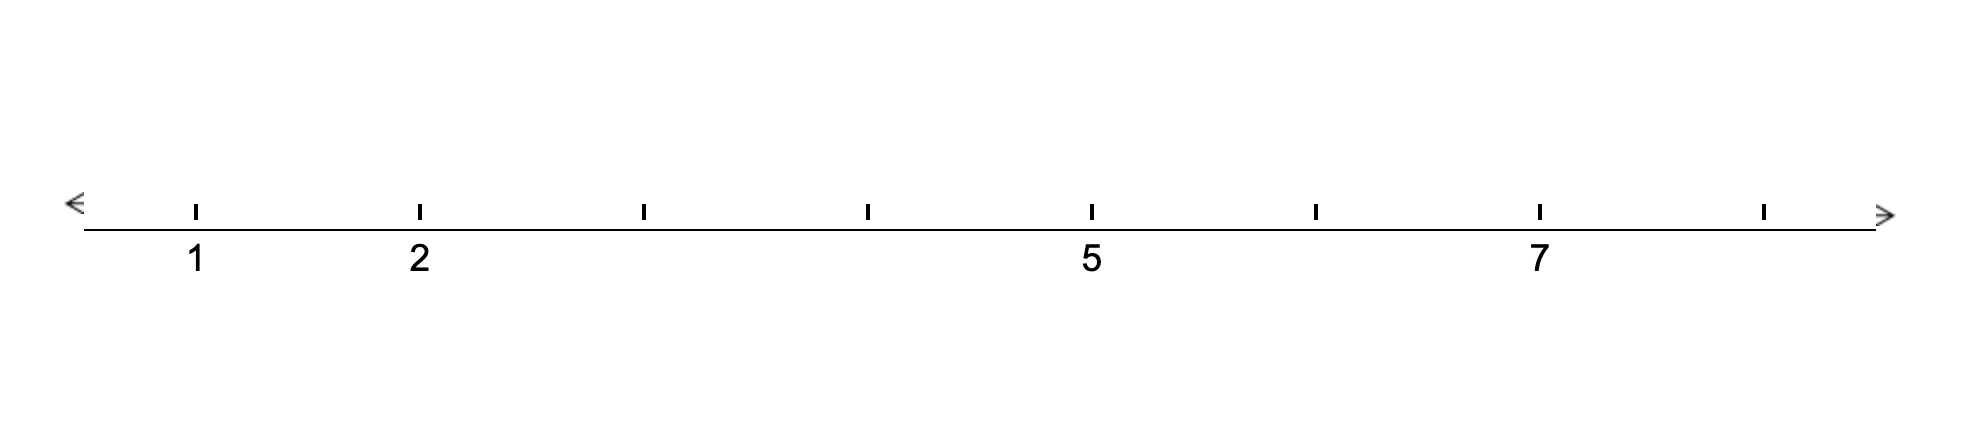
\includegraphics[scale=0.5]{2a.png}
\end{center}

When $K=3$, the optimal clustering solution involves placing the centers at $\mu_{1}=1.5, \mu_{2}=5$, and $\mu_{3}=7$. This arrangement assigns $x_{1}$ and $x_{2}$ to $\mu_{1}$, $x_{3}$ to $\mu_{2}$, and $x_{4}$ to $\mu_{3}$. The value of the objective, then, can be calculated as:

$$
(1-1.5)^{2}+(2-1.5)^{2}+(5-5)^{2}+(7-7)^{2}=0.5
$$

\subsection{(b)}
\sol x A possible suboptimal assignment would be $\mu_{1}=1, \mu_{2}=2$, and $\mu_{3}=6$, where $x_{1}$ is assigned to $\mu_{1}, x_{2}$ is assigned to $\mu_{2}$, and $x_{3}$ and $x_{4}$ are assigned to $\mu_{3}$. The value of the objective is:

$$
(1-1)^{2}+(2-2)^{2}+(5-6)^{2}+(7-6)^{2}=2
$$

The resulting objective value is 2, which is larger than the value of 0.5 obtained in part (a). However, if we apply Lloyd's algorithm to this assignment, we find that $x_{1}$ is closest to $\mu_{1}$, $x_{2}$ is closest to $\mu_{2}$, and both $x_{3}$ and $x_{4}$ are closest to $\mu_{3}$. As a result, there is no change in assignments or centroids. Therefore, we have arrived at a suboptimal solution that represents only a local minimum, rather than the global minimum.

\section{Gaussian Mixture Models}

\subsection{(a)}
\sol x The multivariate normal distribution represents a variable with $d$ dimensions and is characterized by its mean $\boldsymbol{\mu}$ and covariance matrix $\boldsymbol{\Sigma}$. It is given by the formula:

$$
N(\mathbf{x} \mid \boldsymbol{\mu}, \boldsymbol{\Sigma})=\frac{1}{\sqrt{(2 \pi)^{d}|\boldsymbol{\Sigma}|}} \exp \left(-\frac{1}{2}(\mathbf{x}-\boldsymbol{\mu})^{T} \boldsymbol{\Sigma}^{-1}(\mathbf{x}-\boldsymbol{\mu})\right)
$$

After substituting this in the formula for $l(\boldsymbol{\theta})$, the gradient with respect to $\boldsymbol{\mu}_{j}$ is computed as follows:
$$
\begin{gathered}
l(\boldsymbol{\theta})=\sum_{k} \sum_{n} \gamma_{n k} \log \omega_{k}+\sum_{k} \sum_{n} \gamma_{n k} \log \left(\frac{1}{\sqrt{(2 \pi)^{d}\left|\boldsymbol{\Sigma}_{k}\right|}} \exp \left(-\frac{1}{2}\left(\mathbf{x}_{n}-\boldsymbol{\mu}_{k}\right)^{T} \boldsymbol{\Sigma}_{k}^{-1}\left(\mathbf{x}_{n}-\boldsymbol{\mu}_{k}\right)\right)\right. \\
l(\boldsymbol{\theta})=\sum_{k} \sum_{n} \gamma_{n k} \log \omega_{k}+\sum_{k} \sum_{n} \gamma_{n k}\left(\left(\log \frac{1}{\sqrt{(2 \pi)^{d}\left|\boldsymbol{\Sigma}_{k}\right|}}\right)-\frac{1}{2}\left(\mathbf{x}_{n}-\boldsymbol{\mu}_{k}\right)^{T} \boldsymbol{\Sigma}_{k}^{-1}\left(\mathbf{x}_{n}-\boldsymbol{\mu}_{k}\right)\right)
\end{gathered}
$$

The first summation is not a function of $\boldsymbol{\mu}_{\mathrm{j}}$ and the first term in the second summation is constant, which means that their gradients are both equal to zero. Therefore, taking the gradient results in:

$$
\begin{gathered}
\nabla_{\boldsymbol{\mu}_{j}} l(\boldsymbol{\theta})=\frac{\partial}{\partial \boldsymbol{\mu}_{j}} \sum_{n}\left(-\frac{1}{2} \gamma_{n j}\left(\mathbf{x}_{n}-\boldsymbol{\mu}_{j}\right)^{T} \boldsymbol{\Sigma}_{j}^{-1}\left(\mathbf{x}_{n}-\boldsymbol{\mu}_{j}\right)\right) \\
\nabla_{\boldsymbol{\mu}_{j}} l(\boldsymbol{\theta})=\sum_{n}\left(-\frac{1}{2} \gamma_{n j}(2)(-1)\left(\mathbf{x}_{n}-\boldsymbol{\mu}_{j}\right) \boldsymbol{\Sigma}_{j}^{-1}\right) \\
\nabla_{\boldsymbol{\mu}_{j}} l(\boldsymbol{\theta})=\boldsymbol{\Sigma}_{j}^{-1} \sum_{n}\left(\gamma_{n j}\left(\mathbf{x}_{n}-\boldsymbol{\mu}_{j}\right)\right)
\end{gathered}
$$

\subsection{(b)}
\sol x To obtain the desired answer, we set the result obtained in part (a) equal to zero and solve for $\boldsymbol{\mu}_{j}$.

$$
\begin{gathered}
\nabla_{\boldsymbol{\mu}_{j}} l(\boldsymbol{\theta})=\boldsymbol{\Sigma}_{j}^{-1} \sum_{n}\left(\gamma_{n j}\left(\mathbf{x}_{n}-\boldsymbol{\mu}_{j}\right)\right)=\mathbf{0} \\
\sum_{n} \gamma_{n j} \mathbf{x}_{n}=\boldsymbol{\mu}_{j} \sum_{n} \gamma_{n j} \\
\boldsymbol{\mu}_{j}=\frac{\sum_{n} \gamma_{n j} \mathbf{x}_{n}}{\sum_{n} \gamma_{n j}}
\end{gathered}
$$

\subsection{(c)}
\sol x We learned in lecture that we can express $\omega_{k}$ and $\boldsymbol{\mu}_{k}$ as follows:

$$
\omega_{k}=\frac{\sum_{n} \gamma_{n k}}{\sum_{k} \sum_{n} \gamma_{n k}} \quad \boldsymbol{\mu}_{k}=\frac{\sum_{n} \gamma_{n k} \mathbf{x}_{n}}{\sum_{n} \gamma_{n k}}
$$

After substituting the values from the table, we obtain the following values:

$$
\begin{aligned}
& \omega_{1}=\frac{0.2+0.2+0.8+0.9+0.9}{0.2+0.2+0.8+0.9+0.9+0.8+0.8+0.2+0.1+0.1}=\frac{3}{5}=0.6 \\
& \omega_{2}=\frac{0.8+0.8+0.2+0.1+0.1}{5}=\frac{2}{5}=0.4 \\
& \mu_{1}=\frac{1}{3}(0.2(5)+0.2(15)+0.8(25)+0.9(30)+0.9(40))=29 \\
& \mu_{2}=\frac{1}{2}(0.8(5)+0.8(15)+0.2(25)+0.1(30)+0.1(40))=14
\end{aligned}
$$

\end{document}
